\chapter{Drawbacks of Traditional Malware Analysis Methods\label{chap:drawbacks}}

\vspace{4mm}
The drawbacks and some of the methods used to defeat traditional static and dynamic malware analysis methods are discussed below.   
\\
\section{Drawbacks of Static Analysis }
As described in the previous section, static analysis of malware refers to the slew of methods that extract features from a malware program without actually executing it. These features include but are not limited to opcodes, binary representation of the program, function calls and API names. The antivirus program then tries to match a signature from its known database with the binary form of the malware. If a match is found, then it is flagged as a malware. There are efficient string comparison algorithms like Aho-Corasick \cite{Bayer2006}, \cite{4317914} which make this process possible. However, this approach could be defeated by using various code obfuscation techniques. \cite{moser_kruegel_kirda_2007} discusses some of these techniques which include using opaque constants, control flow obfuscation, data location obfuscation and data usage obfuscation. 

\textbf{Opaque constants} - Throughout the malware binary the use of constant values can be seen. They are often used as target of control flows, operand of arithmetic expressions, etc. It is possible to manipulate these constant values by substituting expressions that are semantically equal to the constant value but produce different binary representations \cite{moser_kruegel_kirda_2007}. For example, instead of using constant value take an exclusive or with zero to get an equivalent value. Figure~\ref{fig:OpaqueConstants} shows how a code fragment could be written to manipulate opaque constants.

\begin{center}
	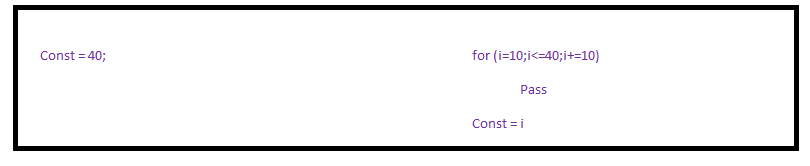
\includegraphics[width=0.80\textwidth]{images/Figure1.png}
	\captionof{figure}{Opaque constants being generated in multiple ways.} 
	\label{fig:OpaqueConstants}
\end{center}


\textbf{Control flow obfuscation} - A control flow graph is defined as a directed graph G = (V,E) in which the vertices represent basic blocks and an edge represents the flow of control between the two vertices \cite{moser_kruegel_kirda_2007}. Unconditional jump and calls could be replaced with a sequence of instructions that perform the same thing but is difficult to determine.

\textbf{Data location obfuscation} - Data elements are located by specifying a constant address. A static analyzer could be misled by using opaque constants for specifying the location and hiding the data elements \cite{moser_kruegel_kirda_2007}.

\textbf{Data usage obfuscation} - Static analyzers are good at identifying the chain of operations that lead to a value being stored in a register, so with data usage obfuscation the idea is to spill values to an obfuscated memory location and then reload it later \cite{moser_kruegel_kirda_2007}.

\cite{sharif2008impeding} discusses techniques like encryption which could also be used for scrambling the binary form of the malware. Encrypting parts of the malware program makes sure that the binary form of it is just a meaningless random combination of zeros and ones. The decryption code then decrypts this encrypted block when the malware is executed. Figure~\ref{fig:CodeDecryption} shows an example of a code fragment decrypting itself based on some condition.

\begin{center}
	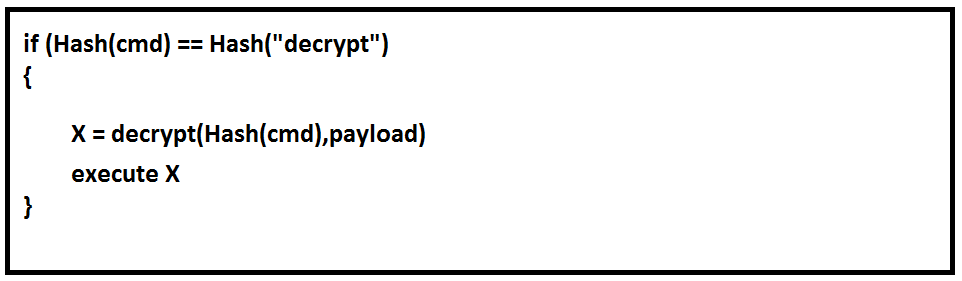
\includegraphics[width=0.80\textwidth]{images/Figure2.png}
	\captionof{figure}{Code decryption based on a command supplied at runtime of the malware.} 
	\label{fig:CodeDecryption}
\end{center}

\cite{5633410} discusses techniques like dead-code insertion, register reassignment, subroutine reordering, code transposition, code integration. 

\textbf{Dead-code insertion} -  This is a very simple mechanism in which the malware writer inserts some random instructions that have no effect on the flow of the program or no operation instructions \cite{5633410}.

\textbf{Register reassignment} - In this technique the register being used is switched around for each generation of then malware \cite{5633410}. Figure~\ref{fig:RegisterReassignment} shows an example of a code fragment that performs register reassignment using the well know EAX, EBX and EDX registers.

\begin{center}
	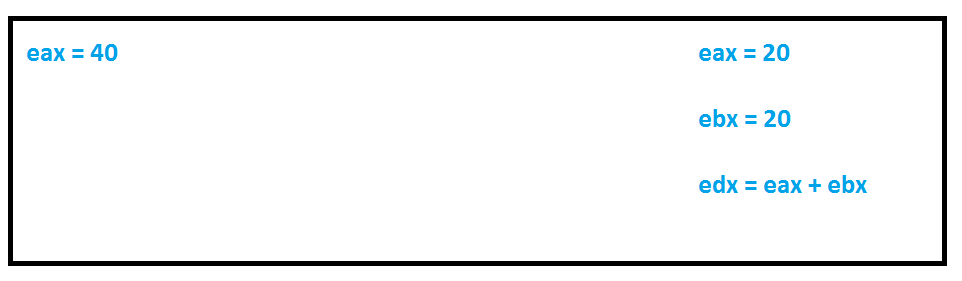
\includegraphics[width=0.80\textwidth]{images/Figure3.png}
	\captionof{figure}{Register reassignment techniques by using multiple registers to achieve same result.} 
	\label{fig:RegisterReassignment}
\end{center}

\textbf{Subroutine reordering} - In this technique the order of the various subroutines is changed in some random order in each malware generation \cite{Bayer2006}.

\textbf{Code transposition} - In this technique the sequence of instructions in the original code are reordered without having an impact on the behavior of the malware \cite{Bayer2006}.

\textbf{Code integration }- In this technique the malware appends itself to the code of its target program, the target being a benign program \cite{Bayer2006}.

The consensus is that malware writers have become wise to the use of signature based detection methods and have begun incorporating various code obfuscation techniques into their malware to evade the antivirus products. Hence, there is a need for a detection mechanism which is robust in the face of code obfuscation techniques.
\\
\section{Drawbacks of Dynamic Analysis }

Analyzing actions performed by a malware while it is running is called dynamic analysis. In dynamic analysis, the malware binary is run in an emulated operating system environment and its security related events are monitored. The windows API calls, native system calls that the program uses are monitored \cite{Egele:2008:SAD:2089125.2089126}. Figure~\ref{fig:IDAPro} shows the usage of IDA Pro software for tracing function calls of a malware script.

\begin{center}
	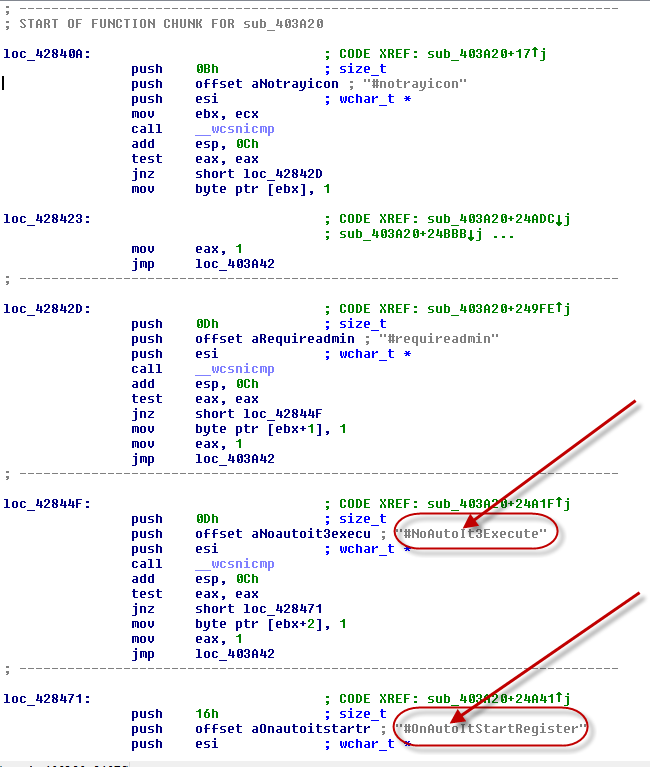
\includegraphics[width=0.80\textwidth]{images/Figure4.png}
	\captionof{figure}{Malware analysis using IDA Pro for extraction of function calls.} 
	\label{fig:IDAPro}
\end{center}

Function call monitoring, function parameter analysis, information flow tracking, instruction trace, AutoStart Extensibility Points(ASEP) are some of the information being collected during dynamic analysis \cite{Egele:2008:SAD:2089125.2089126}.

\textbf{Function call monitoring} - Functions are used to abstract implementation details. For analyzing the behavior of a malware program it is very useful to see what happens in these functions. The process of intercepting functions is called hooking. Once the function is hooked it can be used to analyze the contents of the stack, parameters and so on \cite{Egele:2008:SAD:2089125.2089126}.

\textbf{Function parameter analysis} - Dynamic function parameter analysis is used for getting the arguments that are actually passed to the function during runtime. Tracking these parameters would be useful in finding correlation of individual function calls that operate on the same object \cite{Egele:2008:SAD:2089125.2089126}. This provides a detailed insight into the program’s behavior from an object centric view.

\textbf{Information flow tracking} - The goal of information flow tracking is to track the flow of ‘interesting’ information as the program executes. Taint sources and taint sinks form an important part of this technique. Taint sources are the ones from where tainted data is introduced into the program flow and taint sink is a specific component of the system that reacts in a certain way when simulated with the tainted source \cite{Egele:2008:SAD:2089125.2089126}.

\textbf{Instruction trace} - In this technique a trace of the low level machine instructions is traced as the program executes. This could reveal information that was potentially missed when looking at high level instructions.

\textbf{AutoStart Extensibility Points(ASEP)} - ASEPs provide a mechanism for programs to be automatically invoked upon the operating system boot process \cite{Egele:2008:SAD:2089125.2089126}. Typically, malwares would persist by using these ASEPs.


Though dynamic analysis techniques offer a very good precision in recognizing malware it would not scale well, it takes a lot of time for extracting these features. Since it takes almost close to 3 minutes in some cases, this cannot be used for production cases. Also, it tend to produce a lot of false positives as it finds benign processes which might be making calls that might be out of the norm. 

